%!TEX root = ../../adrien_gomar_phd.tex

Originally developed by \citet{He1998} and \citet{Ning1998},
the 
NonLinear Harmonic method
relies on a decomposition of the conservative variables into a
time-averaged part plus an unsteady perturbation:
\begin{equation}
	u = \overline{u} + u^\prime,
	\label{eq:sm_nlh_decomposition}
\end{equation}
where $\overline{.}$ denotes the time-averaging operator and
$.^\prime$ the corresponding unsteady perturbation.
By injecting Eq.~\ref{eq:sm_nlh_decomposition} into
Eq.~\ref{eq:sm_nonlinear_convection_conservative}, one gets:
\begin{equation}
	\frac{\partial u^\prime}{\partial t} + 
	\frac{1}{2}\frac{\partial}{\partial x} \left[
	\overline{u}^2 + 2 \overline{u} u^\prime + u^\prime u^\prime \right] = 
	0.
	\label{eq:sm_nlh_step_1}
\end{equation}
The time-averaged equation can be obtained by time-averaging
equation~\ref{eq:sm_nlh_step_1}:
\begin{equation}
	(\overline{\ref{eq:sm_nlh_step_1}})
	\Leftrightarrow
	\frac{\partial}{\partial x}
	\left[\overline{u}^2 + 
	\overline{u^\prime u^\prime}\right] =
	0,
	\label{eq:sm_nlh_step_2}
\end{equation}
The term $\overline{u^\prime u^\prime}$
appears due to the non-linearities of the considered equation. It
is called the nonlinear stress terms 
(or the deterministic stress terms) as a reference to 
the Reynolds stress terms. 
The equations for the unsteady perturbations is then obtained by keeping
the first order terms of the unsteady equation~\ref{eq:sm_nlh_step_1}.
This means that the term $u^\prime u^\prime$ is neglected and leads
to:
\begin{equation}
	\frac{\partial u^\prime}{\partial t} + 
	\frac{\partial}{\partial x} \left[\overline{u} u^\prime \right] = 
	0.
\end{equation}

\paragraph{Mono-frequential formulation}
For now on, no assumption has been made neither on the velocity $u$,
nor on its time-averaged part and unsteady perturbation part.
Now, assuming that the velocity perturbation 
is periodic in time with period
$T=2 \pi / \omega$,
the unsteady fluctuations can be decomposed into 
a Fourier series:
\begin{equation}
	u^\prime = \sum_{k=-\infty \atop k \neq 0}^{\infty} 
	\widehat{u}_k e^{i \omega k t}.
	\label{eq:sm_nlh_decomposition_pert}
\end{equation}
Hence, since the complex exponentials forms 
an orthogonal basis, we have for all harmonics 
$-\infty \leq k \leq \infty, \; k \neq 0$:
\begin{equation}
	i \omega k \widehat{u}_k + 
	\frac{\partial}{\partial x} \left[ \overline{u} \widehat{u}_k\right] =
	0.
\end{equation}
One can notice that the time-averaged part has been removed from
the Fourier series through $k \neq 0$.
Each harmonic equation represents now a steady equation as no temporal
derivative is present anymore.

The term $\overline{u^\prime u^\prime}$ remains in the time-averaged
equation and needs to be computed. It can be 
directly worked out when the harmonics are known:
\begin{equation}
	\begin{split}
		u^\prime u^\prime &= 
		\left[
			\sum_{k=-\infty \atop k \neq 0}^{\infty} \widehat{u}_k e^{i \omega k t} 
		\right]
		\left[
			\sum_{k=-\infty \atop k \neq 0}^{\infty} \widehat{u}_k e^{i \omega k t} 
		\right] \\
		&= \sum_{k=-\infty \atop k \neq 0}^{\infty} (\widehat{u}_k)^2
		   e^{i 2 \omega k t} +
		   2 \sum_{j,k=-\infty \atop j \neq k \neq 0}^{\infty} 
		   \widehat{u}_k \widehat{u}_j e^{i \omega (j + k) t} \\
	\end{split}
\end{equation}
Thus,
\begin{equation}
	\begin{split}
		\overline{u^\prime u^\prime} &= 
		\frac{1}{T} \int_{t=0}^{T} \left[ 
			\sum_{k=-\infty \atop k \neq 0}^{\infty} (\widehat{u}_k)^2
		   	e^{i 2 \omega k t} +
		   	2 \sum_{j,k=-\infty \atop j \neq k \neq 0}^{\infty} 
		   	\widehat{u}_k \widehat{u}_j e^{i \omega (j + k) t} 
		\right] dt\\
		&= \frac{2}{T} \int_{t=0}^{T} \sum_{j,k=-\infty \atop j \neq k \neq 0}^{\infty} 
		   	\widehat{u}_k \widehat{u}_j 
		   	e^{i \omega (j + k) t} dt \\
		&= \frac{2}{T} \int_{t=0}^{T} 
			\sum_{k=-\infty \atop k \neq 0}^{\infty} 
			\widehat{u}_k \widehat{u}_{-k}  dt.
	\end{split}
\end{equation}
As $\widehat{u}_k$ and $\widehat{u}_{-k}$ are complex conjugates,
finally $\overline{u^\prime u^\prime}$ is equal to:
\begin{equation}
	\overline{u^\prime u^\prime} = 
	2 \sum_{k=-\infty \atop k \neq 0}^{\infty} |\widehat{u}_k|^2.
	\label{eq:sm_nlh_deterministic_stress_terms}
\end{equation}
This last equation only depends on the computed harmonics, meaning
that no term is modelled. Moreover, this term couple the
time-average with the unsteady perturbations. This is this
terms that is \todo{LUR}

Finally, as computing an infinite number of harmonics is not feasible,
the number of harmonics is truncated at order $N$. 
This is a fare assumption as most
of the physical flows have a finite unsteady spectrum. This
is for sure a reduce order approach. The goal of the spectral
methods being to have a compact representation of the unsteady time
signals. As for a mesh grid convergence, the number of harmonics $N$
is increased until the unsteady representation of the signal is
converged for the variable of interest. The discussion on the
convergence of spectral methods will be detailed later on in sec
\todo{section convergence}.


To summarize, the NonLinear Harmonic
method applied to Eq.~\ref{eq:sm_nonlinear_convection_conservative},
gives $2N + 1$ equations:
\begin{equation}
	\fbox{$
	\begin{cases}
		\displaystyle 
		\frac{\partial}{\partial x}
			\left[\overline{u}^2 + 
			\overline{u^\prime u^\prime}\right] &=
			0, \\
		\displaystyle
		i \omega k \widehat{u}_k + 
			\frac{\partial}{\partial x} 
			\left[ \overline{u} \widehat{u}_k\right] &= 
			0, \: k \in [-N, N], \: k \neq 0,
	\end{cases}
	$}
	\label{eq:sm_nlh_subset_eq}
\end{equation}
coupled by the deterministic stress term $\overline{u^\prime u^\prime}$
defined in Eq.~\ref{eq:sm_nlh_deterministic_stress_terms}.
Three hypothesis lies under these equations:
\begin{itemize}
	\item the unsteady perturbations are periodic in time
	with period $T= 2 \pi / \omega$, 
	meaning that they can be decomposed into a Fourier series,
	\item the high-order cross-coupling terms $u^\prime u^\prime$
	are neglected,
	\item the number of harmonics is set to $N$.
\end{itemize}

\paragraph{Multi-frequential formulation}

In \citet{He2002}, the method is extended to a multi-frequential
perturbation. Instead of writing them
using a Fourier series as defined in Eq.~\ref{eq:sm_nlh_decomposition_pert},
these are written using a sum of harmonics each of which
having a frequency $\omega_k$:
\begin{equation}
	u^\prime = \sum_{k=-N \atop k \neq 0}^{N} 
	\widehat{u}_k e^{i \omega_k t}.
	\label{eq:sm_nlh_decomposition_pert_multi}
\end{equation}
Note that the term $k \omega$ in Eq.~\ref{eq:sm_nlh_decomposition_pert}
is now $\omega_k$ meaning that frequencies can be chosen
arbitrarily. In the paper of \citet{He2002}, no mathematical
framework that allows this decomposition is given. To the author
knowledge, it is only in \cite{JGuedeney2013} that the mathematical
justifications that allows writing 
\ref{eq:sm_nlh_decomposition_pert_multi} are given.
The derivation of the equations are kept the same and the following
$2N+1$ subset of equations are given:
\begin{equation}
	\fbox{$
	\begin{cases}
		\displaystyle 
		\frac{\partial}{\partial x}
			\left[\overline{u}^2 + 
			\overline{u^\prime u^\prime}\right] &=
			0, \\
		\displaystyle
		i \omega_k \widehat{u}_k + 
			\frac{\partial}{\partial x} 
			\left[ \overline{u} \widehat{u}_k\right] &= 
			0, \: k \in [-N, N], \: k \neq 0,
	\end{cases}
	$}
	\label{eq:sm_nlh_subset_eq_multi}
\end{equation}
\todo{pseudo-time ??}
with the coupling deterministic stress term evaluated using the
same equation as for the mono-frequential formulation.
In the multi-frequential formulation, this equation is
not generally true:
\begin{equation}
	\overline{u^\prime u^\prime} = 
	\frac{1}{T} \int_{t=0}^{T} \left[ 
		\sum_{k=-\infty \atop k \neq 0}^{\infty} (\widehat{u}_k)^2
	   	e^{i 2 \omega_k t} +
	   	2 \sum_{j,k=-\infty \atop j \neq k \neq 0}^{\infty} 
	   	\widehat{u}_k \widehat{u}_j e^{i (\omega_j + \omega_k) t} 
	\right] dt.
\end{equation}
In the mono-frequential formulation, the term
\begin{equation}
	\frac{1}{T} \int_{t=0}^{T} (\widehat{u}_k)^2
		e^{i 2 \omega k t} dt
\end{equation}
vanishes for each $k$ as the integral of the
exponential $e^{i 2 \omega k t}$ with respect to $t$
is given by $e^{i 2 \omega k t} / 2 i \omega k$ that is
periodic with period $T$. However, in the multi-frequential
formulation, for some choice of frequencies, the period of all
of these may be difficult or even impossible to define. It
seems that mathematical justifications should be given
to be able to evaluate the deterministic stress term 
using Eq.~\ref{eq:sm_nlh_deterministic_stress_terms}.

\paragraph{Clocking effects}
In \citet{He2002}, the nonlinear harmonic method is extended to
compute all clocking position in one computation. Before
go into details of how this is done, let us explain what is
the clocking effect.
\begin{figure}[htbp]
  \centering 
    \subfigure{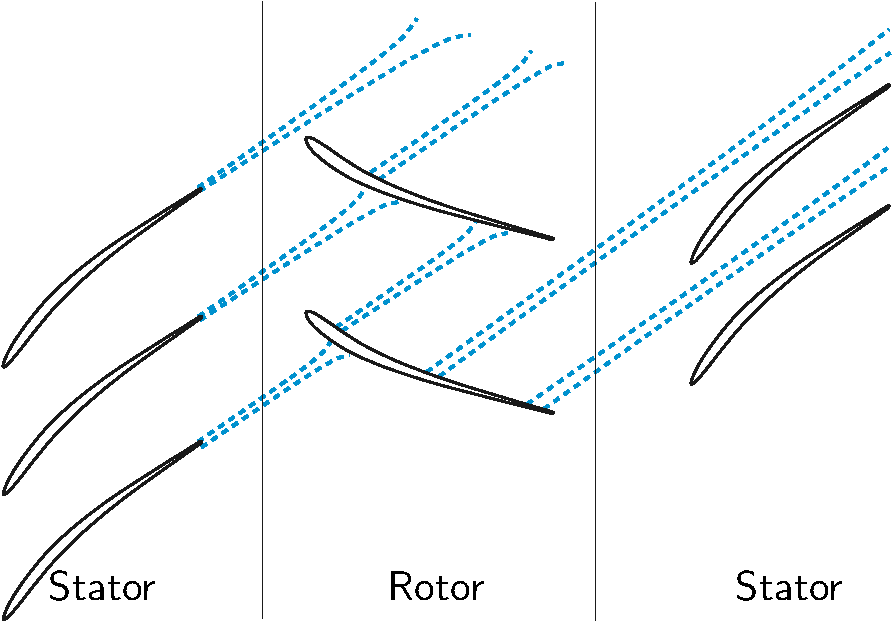
\includegraphics[width=.3\textwidth]{CLOCKING_EFFECT_1.pdf}}
    \subfigure{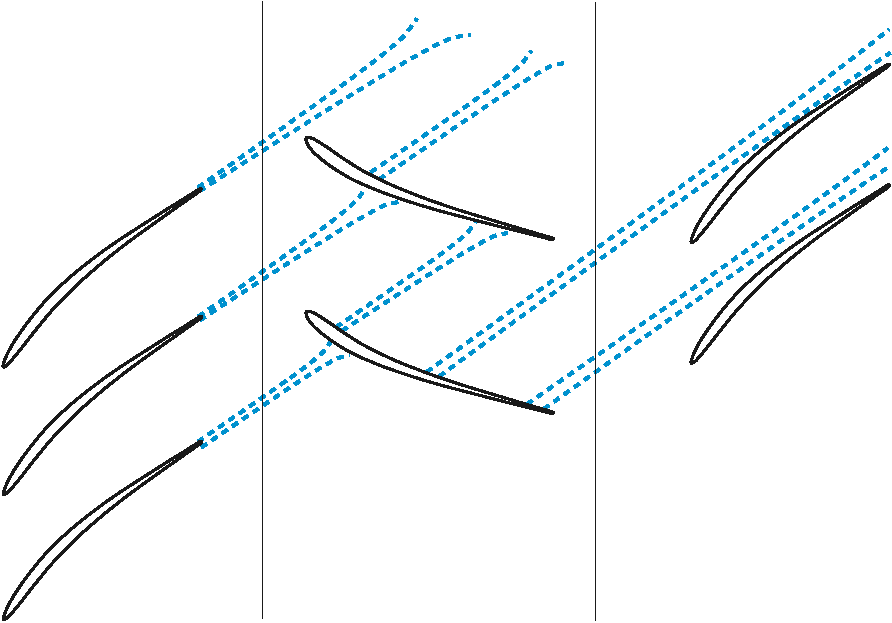
\includegraphics[width=.3\textwidth]{CLOCKING_EFFECT_2.pdf}}
    \subfigure{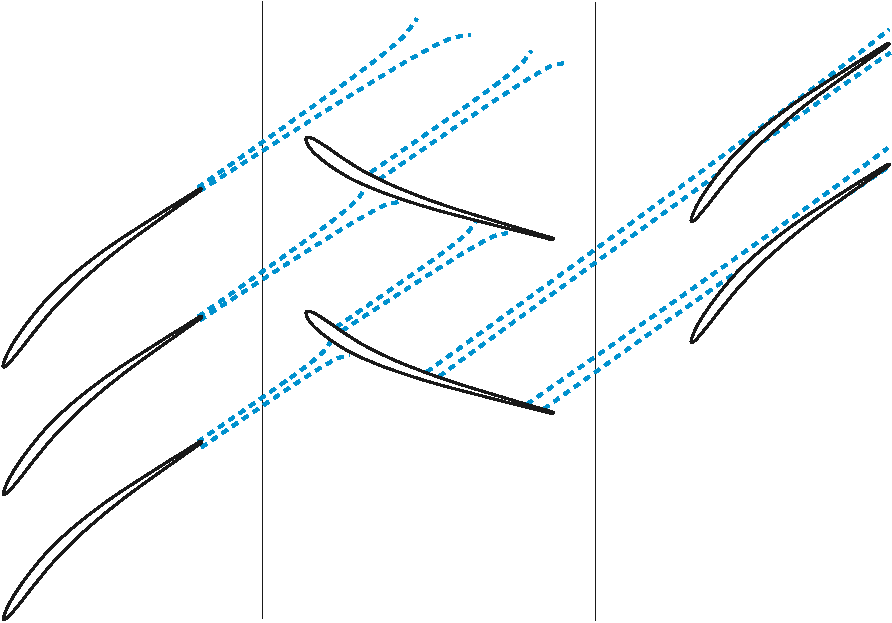
\includegraphics[width=.3\textwidth]{CLOCKING_EFFECT_3.pdf}}
  \caption{Different clocking positions for a stator/rotor/stator
  configuration.}
  \label{fig:sm_nlh_clocking_effect}
\end{figure}
Fig.~\ref{fig:sm_nlh_clocking_effect} displays three subfigures showing three
different clocking position in a stator/rotor/stator configuration.
As both stator are fixed, their relative position is of 
prior interest. The wake that is generated behind the first stator
is cut by the rotor blades but however almost convected up to 
the stator row. The stator being fixed, the wake generated
behind the first stator is seen stationary by the second stator.
Hence, the importance of their relative position. Here, the
first clocking position does not provide unsteadiness to the
last stator while the third clocking position gives the highest
level of unsteadiness for the stator. \todo{papier qui justifie
l'importance du calcul du clocking}

The brute force to compute the clocking effect on a
configuration is to consider all relative positions. This means
that the geometry of the stator should be rotated for each new 
clocking position. The innovative thinking proposed in 
\citet{He2002} is to consider the clocking effect as a steady wave.
In fact, as both stator are fixed, a steady perturbation
generated behind the first stator is still steady in the second stator.
In terms of frequencies, a steady perturbation is a perturbations 
whose frequency is zero. In \citet{He2002} and \cite{Vilmin2009}, 
a perturbation with a very small frequency (close to machine precision)
is computed. The clocking effect can then be evaluated by
post-processing the Fourier coefficient of the zero frequency mode.

Recently, the clocking effects \citet{Vilmin2013a}
\todo{à cmopléter}

\paragraph{Extension to the Navier-Stokes equations}

\paragraph{Applications}
The NonLinear Harmonic method 
has been succesfully implemented
in the NUMECA-Fine/Turbo solver by 
\citet{Vilmin2006, Vilmin2007, Vilmin2009, Vilmin2013a}.\todo{a améliorer + ajout frozen turbulence}

The presented NonLinear Harmonic method is particularly interesting
as it allows to compute the unsteadiness using a small amount 
of steady equations ($2N + 1$, with $N$ the number of harmonics chosen).
However, as all the development have to be made in the frequency domain,
one has to develop a new frequency based CFD solver. To face this issue,
\citet{Hall2002} proposed a new approach, the Harmonic Balance Technique
